\documentclass[final]{beamer}

\usepackage[size=a0,orientation=landscape,scale=1.22]{beamerposter}
\usepackage{tikz}
\usepackage{pgfplots}
\usepackage{qrcode}
\usepackage{booktabs}
\usepackage{amsmath}
\usepackage{amssymb}
\usepackage{listings}
\usetikzlibrary{arrows.meta,positioning,shapes.geometric,calc}
\pgfplotsset{compat=1.18}

\definecolor{BounBlue}{RGB}{0,73,144}
\definecolor{BounLightBlue}{RGB}{229,239,250}
\definecolor{BounPale}{RGB}{246,249,253}
\definecolor{BounDark}{RGB}{30,38,50}
\definecolor{BounGray}{RGB}{245,247,250}
\definecolor{AccentGreen}{RGB}{32,120,103}
\definecolor{AccentOrange}{RGB}{202,103,2}
\definecolor{LeanKeyword}{RGB}{0,77,168}
\definecolor{LeanType}{RGB}{38,127,153}
\definecolor{LeanComment}{RGB}{88,118,71}
\definecolor{LeanBackground}{RGB}{248,248,248}
\definecolor{LeanRule}{RGB}{205,214,224}

\setbeamertemplate{navigation symbols}{}
\setbeamercolor{headline}{fg=white,bg=BounBlue}
\setbeamercolor{block title}{fg=white,bg=BounBlue}
\setbeamercolor{block body}{fg=BounDark,bg=white}
\setbeamercolor{alerted text}{fg=BounBlue}
\setbeamerfont{block title}{size=\Large,series=\bfseries}
\setbeamerfont{block body}{size=\normalsize}

\lstdefinelanguage{Lean}{
  morekeywords={theorem,def,lemma,by,exact,where,namespace,end,variable,import,
    if,then,else,match,with,let,have,show,fun},
  morekeywords=[2]{Domain,CPolynomial,FastMul,Raw,R,Nat,Array},
  morekeywords=[3]{fastMulImpl,fastMulSpec,safeFastMul,fits,val,mul},
  sensitive=true,
  morecomment=[l]--,
  morestring=[b]"
}

\lstset{
  language=Lean,
  basicstyle=\ttfamily\small,
  keywordstyle=\color{LeanKeyword}\bfseries,
  keywordstyle=[2]\color{LeanType},
  keywordstyle=[3]\color{AccentGreen},
  commentstyle=\color{LeanComment},
  stringstyle=\color{AccentOrange},
  columns=fullflexible,
  keepspaces=true,
  showstringspaces=false,
  breaklines=true,
  frame=single,
  framerule=0.8pt,
  rulecolor=\color{LeanRule},
  backgroundcolor=\color{LeanBackground},
  xleftmargin=0.35cm,
  xrightmargin=0.35cm,
  aboveskip=0.35cm,
  belowskip=0.25cm
}

\newcommand{\projecttitle}{Formal Verification of Number-Theoretic Transform in Lean}
\newcommand{\leaninline}[1]{\texttt{#1}}

\newenvironment{posterblock}[1]{%
  \begin{block}{#1}
  \vspace{0.35em}
}{%
  \vspace{0.25em}
  \end{block}
}

\newcommand{\complexityTable}{%
\begin{center}
\renewcommand{\arraystretch}{1.16}
\resizebox{0.94\linewidth}{!}{%
\begin{tabular}{@{}lll@{}}
\toprule
\textbf{Method} & \textbf{Main Operation} & \textbf{Work} \\
\midrule
Naive & sum coefficient pairs & $O(n^2)$ \\
NTT & transform, pointwise multiply, transform back & $O(n\log n)$ \\
\bottomrule
\end{tabular}
}%
\end{center}
}

\newcommand{\nttDiagram}{%
\resizebox{0.985\linewidth}{!}{%
\begin{tikzpicture}[
  node distance=1.3cm and 1.2cm, % Defines standard vertical and horizontal gaps
  coeff/.style={draw=BounBlue, line width=1.15pt, rounded corners=4pt, fill=BounPale,
    align=center, inner sep=8pt, minimum width=5.7cm, minimum height=1.42cm, font=\normalsize},
  eval/.style={draw=AccentGreen, line width=1.15pt, rounded corners=4pt, fill=white,
    align=center, inner sep=8pt, minimum width=5.9cm, minimum height=1.42cm, font=\normalsize},
  point/.style={draw=AccentOrange, line width=1.15pt, rounded corners=4pt, fill=white,
    align=center, inner sep=9pt, minimum width=5.9cm, minimum height=1.85cm, font=\normalsize},
  product/.style={draw=BounBlue, line width=1.15pt, rounded corners=4pt, fill=BounPale,
    align=center, inner sep=9pt, minimum width=6.2cm, minimum height=1.75cm, font=\normalsize},
  stage/.style={draw=BounBlue, fill=BounBlue, text=white, line width=1pt,
    rounded corners=3pt, align=center, font=\bfseries\normalsize,
    minimum width=2.1cm, minimum height=0.88cm},
  domainlabel/.style={font=\bfseries\large},
  arrow/.style={-{Latex[length=3.5mm]}, line width=1.12pt, draw=BounBlue}
]

% --- Left side: Forward Transforms ---
% Row 1
\node[coeff] (pcoeff) {$p(x)=a_0+a_1x+\cdots$};
\node[stage, right=of pcoeff] (pntt) {NTT};
\node[eval, right=of pntt] (phat) {$\widehat p=[p(\omega^i)]_{i<n}$};

% Row 2 (Positioned neatly below Row 1)
\node[coeff, below=of pcoeff] (qcoeff) {$q(x)=b_0+b_1x+\cdots$};
\node[stage, right=of qcoeff] (qntt) {NTT};
\node[eval, right=of qntt] (qhat) {$\widehat q=[q(\omega^i)]_{i<n}$};

% --- Middle: Pointwise Product ---
% Anchor to the exact vertical midpoint of phat and qhat
\path ($(phat.east)!0.5!(qhat.east)$) ++(1.8cm, 0) node[point, anchor=west] (prodValues) {%
  \textbf{pointwise product}\\[0.15em]
  $\widehat c=\widehat p\odot\widehat q$\\[-0.05em]
  $\widehat c_i=\widehat p_i\widehat q_i$};

% --- Right side: Inverse Transform ---
\node[stage, minimum width=3.0cm, right=of prodValues] (intt) {inverse\\NTT};
\node[product, right=of intt] (product) {%
  $c(x)=p(x)q(x)$\\[0.3em]
  $c_k=\sum_{i+j=k} a_i b_j$};

% --- Headers ---
% Use coordinate projection (A -| B) to perfectly align horizontally with the nodes 
% and vertically with the first label.
\node[domainlabel, text=BounBlue, above=1.2cm of pcoeff] (label1) {coefficient inputs};
\node[domainlabel, text=AccentGreen] at (label1 -| phat) {evaluation domain};
\node[domainlabel, text=BounBlue] at (label1 -| product) {coefficient output};

% --- Arrows ---
\draw[arrow] (pcoeff) -- (pntt);
\draw[arrow] (pntt) -- (phat);
\draw[arrow] (qcoeff) -- (qntt);
\draw[arrow] (qntt) -- (qhat);

% Cleanly route arrows to the upper and lower halves of the product node
\draw[arrow] (phat.east) -- ([yshift=0.4cm]prodValues.west);
\draw[arrow] (qhat.east) -- ([yshift=-0.4cm]prodValues.west);

\draw[arrow] (prodValues) -- (intt);
\draw[arrow] (intt) -- (product);

\end{tikzpicture}%
}%
}

\newcommand{\moduleDiagram}{%
\resizebox{0.93\linewidth}{!}{%
\begin{tikzpicture}[
  node distance=0.8cm,
  main/.style={draw=BounBlue, line width=1.1pt, rounded corners=4pt, fill=BounPale,
    align=center, minimum width=12.5cm, minimum height=1.55cm},
  tag/.style={draw=none, rounded corners=3pt, fill=BounBlue, text=white,
    font=\bfseries\small, align=center, minimum width=3.0cm, minimum height=0.9cm},
  arrow/.style={-{Latex[length=3mm]}, line width=1pt, draw=BounBlue}
]
\node[main] (domain) {\textbf{Domain}\\size, root of unity, inverse root};
\node[main, below=of domain] (transform) {\textbf{Forward / Inverse Transform}\\iterative radix-2 butterfly implementation};
\node[main, below=of transform] (pipeline) {\textbf{FastMul.Raw}\\forward transform, pointwise multiplication, inverse transform};
\node[main, below=of pipeline] (api) {\textbf{FastMul}\\canonical \leaninline{CPolynomial} result};
\node[tag, left=0.55cm of domain] {parameters};
\node[tag, left=0.55cm of transform] {algorithm};
\node[tag, left=0.55cm of pipeline] {pipeline};
\node[tag, left=0.55cm of api] {public API};
\draw[arrow] (domain) -- (transform);
\draw[arrow] (transform) -- (pipeline);
\draw[arrow] (pipeline) -- (api);
\end{tikzpicture}%
}%
}

\newcommand{\benchmarkPlot}{%
\begin{tikzpicture}
\begin{axis}[
  width=0.90\linewidth,
  height=8.5cm,
  grid=both,
  major grid style={draw=LeanRule},
  minor grid style={draw=LeanRule!55},
  xlabel={operand size $n$},
  ylabel={average time (ms)},
  xlabel style={font=\large},
  ylabel style={font=\large},
  tick label style={font=\small},
  xmin=64,
  xmax=3200,
  ymin=0,
  ymax=17000,
  scaled y ticks=false,
  xtick={64,512,1024,1536,2048,2560,3000},
  xticklabels={64,512,1024,1536,2048,2560,3000},
  xticklabel style={font=\scriptsize},
  ytick={0,4000,8000,12000,16000},
  yticklabels={0,4000,8000,12000,16000},
  legend style={font=\small, draw=none, fill=white, at={(0.03,0.97)}, anchor=north west},
  legend cell align=left
]
\addplot+[BounBlue, line width=2.0pt, mark=*, mark size=2.2pt]
  coordinates {
    (64,0.25) (96,0.55) (128,0.60) (192,5.00) (256,4.80)
    (384,10.40) (512,10.40) (768,55.50) (1024,59.00)
    (1536,121.50) (2048,241.00) (2560,526.00) (3000,539.00)
  };
\addlegendentry{NTT}
\addplot+[AccentOrange, line width=2.0pt, mark=square*, mark size=2.1pt]
  coordinates {
    (64,0.35) (96,0.85) (128,1.50) (192,12.80) (256,22.80)
    (384,51.00) (512,91.00) (768,518.00) (1024,917.00)
    (1536,2047.00) (2048,7323.00) (2560,11532.00) (3000,15756.00)
  };
\addlegendentry{naive raw}
\end{axis}
\end{tikzpicture}
}

\newcommand{\proofLadder}{%
\resizebox{0.98\linewidth}{!}{%
\begin{tikzpicture}[
  node distance=0.72cm,
  layer/.style={draw=BounBlue, line width=1.05pt, rounded corners=4pt, fill=BounPale,
    align=left, text width=20.5cm, inner sep=7pt, minimum height=1.2cm, font=\small},
  final/.style={draw=AccentGreen, line width=1.3pt, rounded corners=4pt, fill=white,
    align=left, text width=20.5cm, inner sep=7pt, minimum height=1.2cm, font=\small},
  tag/.style={draw=none, fill=BounBlue, text=white, rounded corners=3pt,
    font=\bfseries\scriptsize, align=center, text width=4.2cm, minimum height=0.78cm},
  arrow/.style={-{Latex[length=3.2mm]}, line width=1.05pt, draw=BounBlue}
]
\node[layer] (loops) {\textbf{Executable loops}\\bit reversal and butterfly stages over arrays};
\node[layer, below=of loops] (impl) {\textbf{Implementation refinement}\\\leaninline{forwardImpl\_correct} and \leaninline{inverseImpl\_correct}};
\node[layer, below=of impl] (spec) {\textbf{Direct NTT specifications}\\root-of-unity summation formulas for forward and inverse transforms};
\node[layer, below=of spec] (eval) {\textbf{Evaluation-domain algebra}\\pointwise products match evaluation of $p(x)q(x)$};
\node[layer, below=of eval] (fit) {\textbf{No wraparound under \leaninline{Domain.fits}}\\the chosen domain is large enough for the convolution length};
\node[final, below=of fit] (result) {\textbf{Public theorem}\\\leaninline{fastMulImpl\_eq\_mul}: canonical fast multiplication equals $p*q$};

\node[tag, left=0.5cm of loops] {code};
\node[tag, left=0.5cm of impl] {refinement};
\node[tag, left=0.5cm of spec] {spec};
\node[tag, left=0.5cm of eval] {algebra};
\node[tag, left=0.5cm of fit] {shape};
\node[tag, left=0.5cm of result, fill=AccentGreen] {result};

\draw[arrow] (loops) -- (impl);
\draw[arrow] (impl) -- (spec);
\draw[arrow] (spec) -- (eval);
\draw[arrow] (eval) -- (fit);
\draw[arrow] (fit) -- (result);
\end{tikzpicture}%
}%
}

\begin{document}

\begin{frame}[fragile,t]

\vspace*{-0.22cm}
\begin{beamercolorbox}[wd=\paperwidth,sep=1.15cm]{headline}
  \begin{columns}[c,totalwidth=\paperwidth]
    \begin{column}{0.12\paperwidth}
      \centering
      
\includegraphics[height=5.8cm]{boun_logo.eps}
    \end{column}
    \begin{column}{0.76\paperwidth}
      \centering
      {\bfseries\fontsize{58}{66}\selectfont \projecttitle\par}
      \vspace{0.42cm}
      {\Large Salih Erdem Ko\c{c}ak, Doran Pamuk\c{c}u\par}
      \vspace{0.18cm}
      {\large Advisor: Do\u{g}an Ulus \quad Department of Computer Engineering, Bo\u{g}azi\c{c}i University\par}
    \end{column}
    \begin{column}{0.12\paperwidth}
      \centering
      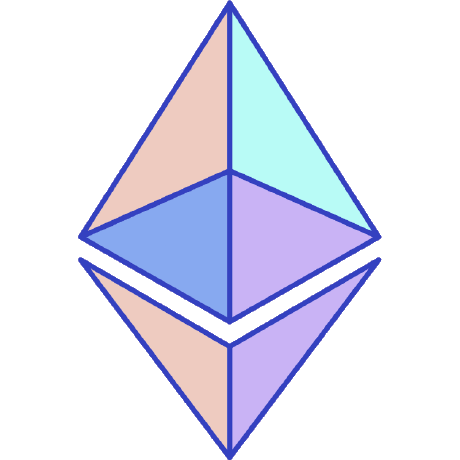
\includegraphics[height=5.8cm]{verified_zkevm_logo_transparent.png}
    \end{column}
  \end{columns}
\end{beamercolorbox}

\vspace{0.85cm}

\begin{columns}[T,totalwidth=0.96\paperwidth]

\begin{column}{0.63\paperwidth}

\begin{columns}[T,totalwidth=\linewidth]
\begin{column}{0.49\linewidth}

\begin{posterblock}{Motivation}
Polynomial multiplication is a core component of many cryptographic protocols, especially proof systems. Evaluation and interpolation routines, polynomial commitments, and quotient-polynomial constructions all multiply polynomials repeatedly. With the usual schoolbook algorithm, this is quadratic work. The NTT avoids direct convolution by evaluating both inputs on a root-of-unity domain, multiplying the values pointwise, and then transforming back. Our Lean proof connects this executable pipeline to the algebraic specification, showing that the fast path is correct.

\vspace{0.9cm}
\complexityTable
\end{posterblock}

\end{column}
\begin{column}{0.49\linewidth}

\begin{posterblock}{Implementation Surface}
\centering
\moduleDiagram

\vspace{0.65em}
The public operation is small; most of the work is in connecting executable array code to mathematical transform specifications and then to polynomial multiplication.
\end{posterblock}

\end{column}
\end{columns}

\vspace{0.45cm}

\begin{posterblock}{NTT Multiplication}
\centering
\nttDiagram

\vspace{0.55em}
{\large The transform evaluates at powers of a root of unity. Multiplication becomes pointwise in the evaluation domain, then the inverse transform returns the coefficient representation.}
\end{posterblock}

\vspace{0.45cm}

\begin{columns}[T,totalwidth=\linewidth]
\begin{column}{0.49\linewidth}

\begin{posterblock}{Benchmark Behavior}
\centering
\benchmarkPlot

\vspace{-0.2cm}
{\small Manual KoalaBear benchmark sweep from \leaninline{tests/CompPolyTests/Univariate/NTT/Benchmark.lean}. Times are illustrative and machine-dependent.}
\end{posterblock}

\end{column}
\begin{column}{0.49\linewidth}

\begin{posterblock}{Main Theorem}
\begin{lstlisting}[basicstyle=\ttfamily\normalsize]
theorem fastMulImpl_eq_mul
    (D : Domain R)
    (p q : CPolynomial R)
    (hfit : Domain.fits D p.val q.val) :
    fastMulImpl D p q = p * q
\end{lstlisting}

This is the public correctness statement for the multiplication implementation. The precondition
\leaninline{Domain.fits D p.val q.val} says that the selected NTT domain is large enough for the
ordinary convolution, so the transform pipeline has no cyclic wraparound.
\end{posterblock}

\end{column}
\end{columns}

\end{column}

\begin{column}{0.31\paperwidth}

\begin{posterblock}{Proof Architecture}
\centering
\proofLadder
\end{posterblock}

\begin{posterblock}{References}
\begin{enumerate}\small
  \setlength{\itemsep}{0.22em}
  \item Trieu, A., ``Formally Verified Number-Theoretic Transform.'' \textit{IACR Communications in Cryptology}, vol. 2, no. 4, Jan. 2026. DOI: \texttt{10.62056/ahbn-4tw9}.
  \item Capretta, V., ``Certified Fast Fourier Transform.'' \textit{Theorem Proving in Higher Order Logics}, TPHOLs 2001. Springer, 2001.
  \item Ballarin, C., ``Fast Fourier Transform.'' \textit{Archive of Formal Proofs}, Oct. 2005. \texttt{isa-afp.org/entries/FFT.html}.
  \item Truth Research ZK, ``AMO-Lean'', 2026. \texttt{github.com/lambdaclass/amo-lean}.
\end{enumerate}
\end{posterblock}

\begin{posterblock}{Code and Repository}
\begin{columns}[T,totalwidth=\linewidth]
  \begin{column}{0.48\linewidth}
    \centering
    \qrcode[height=5.1cm]{https://github.com/Verified-zkEVM/CompPoly/pull/174}

    \vspace{0.22cm}
    \textbf{Merged PR \#174}
  \end{column}
  \begin{column}{0.48\linewidth}
    \centering
    \qrcode[height=5.1cm]{https://github.com/Verified-zkEVM/CompPoly}

    \vspace{0.22cm}
    \textbf{CompPoly Repository}
  \end{column}
\end{columns}
\end{posterblock}

\end{column}

\end{columns}

\end{frame}

\end{document}
